\documentclass[12pt,a4paper]{article}
\usepackage{polyglossia}
\setmainlanguage{russian}
\setotherlanguage{english}
\setmainfont{DejaVu Serif}
\setsansfont{DejaVu Sans}
\setmonofont[Scale=0.88]{DejaVu Sans Mono}
\usepackage{amsmath,amssymb,amsthm}
\usepackage[top=2.5cm,bottom=2.5cm,left=3cm,right=2cm]{geometry}
\usepackage{indentfirst}
\setlength{\parindent}{1.25cm}
\usepackage{graphicx,float,booktabs}
\usepackage[hidelinks]{hyperref}
\usepackage{fancyhdr,enumitem,xcolor,tcolorbox}
\tcbuselibrary{skins}
\setlength{\headheight}{15pt}
\pagestyle{fancy}\fancyhf{}
\rhead{Лабораторная работа 1}\lhead{Вариант 23}\cfoot{\thepage}
\newtheorem{theorem}{Теорема}
\newtheorem{definition}{Определение}

% rating box style
\tcbset{ratingbox/.style={enhanced,colback=yellow!10,colframe=orange!70!black,
  fonttitle=\bfseries,title=Оценка работы,arc=4pt}}

\begin{document}

%──────────────────────────────────────────────
%  ТИТУЛЬНАЯ СТРАНИЦА
%──────────────────────────────────────────────


\begin{titlepage}
\centering
\textbf{Санкт-Петербургский Национальный Исследовательский Университет ИТМО}\\
\textbf{Факультет Программной Инженерии и Компьютерной Техники}

\vspace{2cm}

\includegraphics[width=0.4\textwidth]{ITMOLogo.png}

\vspace{2cm}

{Лабораторная работа №1\\[12pt]
Дисциплина: Математический анализ\\[18pt]
Определённый интеграл Римана\\[18pt]
{Вариант 23}\\[12pt]
}

\vfill

\begin{flushright}
Выполнили студенты:\\
Эллити Мохамед Эмад Ахмед Авад\\
Карецкая Алиса Борисовна\\
Хаммад Али\\

Преподаватели:\\
Рыбинская Злата Владиславовна\\
Романова Екатерина Владимировна
\end{flushright}

\vspace{1.5cm}
Санкт-Петербург, 2026
\end{titlepage}

%==============================================
\section{Постановка задачи}
%==============================================

Дана функция
\[
  f(x)=4^x,\qquad x\in[1,2].
\]
Требуется:
\begin{enumerate}[label=\textbf{\arabic*.}]
  \item Построить верхнюю и нижнюю суммы Дарбу для равномерного разбиения на $n$ частей.
  \item Доказать, что функция интегрируема по Риману.
  \item Найти пределы сумм Дарбу, найти значение интеграла.
  \item Сравнить со значением, полученным по формуле Ньютона--Лейбница.
  \item Численно проверить для $n=5,10,100$; построить графики и таблицу.
\end{enumerate}

%==============================================
\section{Теория}
%==============================================
\subsection{Разбиение отрезка}
\begin{definition}[Stewart, \S 5.1]
\emph{Разбиением} отрезка $[a,b]$ называется набор точек
$P=\{x_0,x_1,\ldots,x_n\}$, $a=x_0<x_1<\cdots<x_n=b$.
Длина $i$-го подотрезка: $\Delta x_i=x_i-x_{i-1}$.
\end{definition}

\noindent\textbf{Равномерное разбиение:}
$\Delta x=\dfrac{b-a}{n}$, $x_k=a+k\cdot\Delta x$.

\subsection{Суммы Дарбу}
\begin{definition}[Stewart, \S 5.1, Def.~2]
Пусть $m_k=\inf_{[x_{k-1},x_k]}f$, $M_k=\sup_{[x_{k-1},x_k]}f$.

\textbf{Нижняя сумма Дарбу:}\;
$s_n = \displaystyle\sum_{k=1}^{n}m_k\,\Delta x$.\\[4pt]
\textbf{Верхняя сумма Дарбу:}\;
$S_n = \displaystyle\sum_{k=1}^{n}M_k\,\Delta x$.
\end{definition}

Всегда: $s_n\leq\int_a^b f\,dx\leq S_n$.

\subsection{Интегрируемость по Риману}
\begin{definition}[Stewart, \S 5.2]
$f$ \emph{интегрируема по Риману}, если
$\sup_P s(f,P)=\inf_P S(f,P)$.
\end{definition}

\begin{theorem}[Критерий Дарбу]
$f$ интегрируема $\Leftrightarrow$ $\forall\varepsilon>0\;\exists P:\;S(f,P)-s(f,P)<\varepsilon$.
\end{theorem}

\begin{theorem}[Stewart, \S 5.2, Th.~3]
Непрерывная на $[a,b]$ функция интегрируема по Риману.
\end{theorem}

\subsection{Интеграл как предел}
\[
  \int_a^b f(x)\,dx=\lim_{n\to\infty}\sum_{k=1}^{n}f(x_k^*)\,\Delta x,
  \qquad x_k^*\in[x_{k-1},x_k].
\]

\subsection{Формула Ньютона--Лейбница}
\begin{theorem}[ФОИ ч.~2; Stewart, \S 5.3, Th.~4]
Если $F'=f$ и $f$ непрерывна на $[a,b]$, то
$\int_a^b f(x)\,dx=\bigl[F(x)\bigr]_a^b=F(b)-F(a)$.
\end{theorem}

%==============================================
\section{Аналитическая часть}
%==============================================

\subsection*{Исходные данные и разбиение}
\begin{itemize}
\item Построить верхнюю и нижнюю суммы Дарбу для равномерного разбиения на n частей.
\item Доказать, что функция интегрируема по Риману.
\item Найти пределы сумм Дарбу, найти значения интеграла.
\item Сравнить со значением, полученным по формуле Ньютона-Лейбница.
\end{itemize}\\
\subsection{Построить верхнюю и нижнюю суммы Дарбу для равномерного разбиения на n частей}

Шаг разбиения:
\[
  \Delta x = \frac{2-1}{n} = \frac{1}{n}.
\]
Точки разбиения:
\[
  x_k = 1+k\cdot\frac{1}{n},\quad k=0,1,\ldots,n.
\]
На каждом подынтервале $[x_{k-1},x_k]$ функция $f(x)=4^x$ \textbf{строго возрастает}
(так как $f'(x)=4^x\ln 4>0$), поэтому:
\begin{itemize}
  \item нижняя сумма $s_n$: берём значение в \emph{левом} конце $f(x_{k-1})$,
  \item верхняя сумма $S_n$: берём значение в \emph{правом} конце $f(x_k)$.
\end{itemize}

%----------------------------------------------
\subsubsection{Шаг 1 --- Построение сумм Дарбу}
%----------------------------------------------

\subsubsection*{Нижняя сумма $s_n$}

\[
  s_n = \sum_{k=1}^{n}f(x_{k-1})\cdot\Delta x
      = \frac{1}{n}\sum_{k=1}^{n}4^{x{1-k}}.
      = \frac{1}{n}\sum_{k=1}^{n}4^{1+\frac{k-1}{n}}.
\]

Вынесем $4^1=4$:
\[
  s_n = \frac{4}{n}\sum_{k=1}^{n}4^{\frac{k-1}{n}}.
\]

$q = 4^1/n \Rightarrow 4^{(k-1)/n} \Rightarrow {(4^{1/n})}^{k-1} = q^{k-1}$

\[
  s_n = \frac{4}{n}\sum_{j=0}^{n-1}q^j
\]
\textbf{Сумма геометрической прогрессии:}
\[
  \sum_{j=0}^{n-1}q^j = \frac{q^n-1}{q-1}.
\]

\text{Но} $q^n = (4^{\frac{1}{n})^n} = 4$
$q^n=\bigl(4^{1/n}\bigr)^n=4$:
\[
  s_n = \frac{4}{n}\cdot\frac{4-1}{4^{1/n}-1}
      = \frac{4}{n}\cdot\frac{3}{4^{1/n}-1}.
\]

\[
  \boxed{s_n = \frac{12}{n\bigl(4^{1/n}-1\bigr)}.}
\]

\subsubsection*{Верхняя сумма $S_n$}

\[
  S_n = \frac{1}{n}\sum_{k=1}^{n}f(x_k)
      = \frac{4}{n}\sum_{k=1}^{n}4^{k/n}
      = \frac{4}{n}\sum_{k=1}^{n}q^k
      = \frac{4}{n}\cdot q\cdot\frac{q^n-1}{q-1}
      = \frac{4}{n}\cdot\frac{3q}{q-1}.
\]


\[
  \boxed{S_n = \frac{12\cdot 4^{1/n}}{n\bigl(4^{1/n}-1\bigr)} = s_n\cdot 4^{1/n}.}
\]

\subsubsection*{В итоге получаем}
\[
    \boxed{s_n = \frac{12}{n\bigl(4^{1/n}-1\bigr)} 
      \   S_n = \frac{12\cdot 4^{1/n}}{n\bigl(4^{1/n}-1\bigr)} = s_n\cdot 4^{1/n}.}
\]
\subsubsection{Кстати}
\[
S_n = s_n \cdot 4^{\frac{1}{n}}
\]
%----------------------------------------------
\subsection*{2. Доказательство интегрируемости}

Функция $f(x)$ интегрируема по Риману на отрезке $[a, b]$ тогда и только тогда, когда для любого $\varepsilon > 0$ существует разбиение $P$ отрезка $[a, b]$ такое, что
\[
S(f, P) - s(f, P) < \varepsilon,
\]
где $S(f, P)$ и $s(f, P)$ --- верхняя и нижняя суммы Дарбу.

Также, стоит учесть, что непрерывная на отрезке функция интегрируема по Риману.

\begin{itemize}
    \item \textbf{Непрерывность.} Функция $4^x$ является показательной. Показательная функция непрерывна на всей числовой прямой, в частности, она непрерывна на отрезке $[1, 2]$.
    \item \textbf{Теорема об интегрируемости непрерывных функций.} Известно, что любая функция, непрерывная на отрезке, интегрируема по Риману на этом отрезке. Это следует из того, что непрерывная на отрезке функция ограничена и равномерно непрерывна.
    \item \textbf{Проверка по критерию Дарбу.} Возьмем произвольное $\varepsilon > 0$. В силу равномерной непрерывности функции на $[1, 2]$, существует такое $\delta > 0$, что для любых $x, y \in [1, 2]$ с $|x - y| < \delta$ выполняется $|f(x) - f(y)| < \varepsilon$. Выберем равномерное разбиение отрезка $[1, 2]$ на $n$ частей с шагом $\Delta x = \frac{1}{n}$ так, чтобы $\Delta x < \delta$. На каждом подынтервале $[x_{k-1}, x_k]$ колебание функции $M_k - m_k < \varepsilon$. Тогда разность верхней и нижней сумм Дарбу:
    \[
    S - s = \sum_{k=1}^{n} (M_k - m_k) \Delta x_k < \sum_{k=1}^{n} \varepsilon \cdot \frac{1}{n} = \varepsilon.
    \]
    \[
    S_n - s_n = s_n(4^{1/n} - 1) = \frac{12}{n(4^{1/n} - 1)} \cdot (4^{1/n} - 1) = \frac{12}{n}.
    \]
    При $n \to \infty$ величина $\frac{12}{n} \to 0$. По критерию Дарбу функция интегрируема.
\end{itemize}

\subsection*{3. Пределы сумм Дарбу}

Из предыдущего вывода:
\[
s_n = \frac{12}{n(4^{1/n} - 1)}, \quad S_n = \frac{12 \cdot 4^{1/n}}{n(4^{1/n} - 1)}.
\]
Найдём $\lim\limits_{n\to\infty} s_n$.

Используем эквивалентность при $n \to \infty$:
\[
4^{1/n} = e^{\ln 4 / n} = 1 + \frac{\ln 4}{n} + o\!\left(\frac{1}{n}\right),
\]
\[
4^{1/n} - 1 \sim \frac{\ln 4}{n}.
\]
Подставляем в $s_n$:
\[
s_n = \frac{12}{n \cdot \left( \frac{\ln 4}{n} + o\!\left(\frac{1}{n}\right) \right)} = \frac{12}{\ln 4 + o(1)} \to \frac{12}{\ln 4}.
\]
Для $S_n$:
\[
S_n = s_n \cdot 4^{1/n} \to \frac{12}{\ln 4} \cdot 1 = \frac{12}{\ln 4}.
\]
Таким образом:
\[
\lim_{n \to \infty} s_n = \lim_{n \to \infty} S_n = \frac{12}{\ln 4}.
\]
По определению интеграла Римана:
\[
\int_{1}^{2} 4^x \, dx = \lim_{n \to \infty} s_n = \lim_{n \to \infty} S_n = \frac{12}{\ln 4}.
\]

\subsection*{4. По формуле Ньютона-Лейбница}
\[
\int_{1}^{2} 4^x \, dx = \frac{4^x}{\ln 4} \bigg|_{1}^{2} = \frac{4^2}{\ln 4} - \frac{4^1}{\ln 4} = \frac{16 - 4}{\ln 4} = \frac{12}{\ln 4}.
\]
Пределы сумм Дарбу:
\[
\lim_{n \to \infty} s_n = \frac{12}{\ln 4}, \quad \lim_{n \to \infty} S_n = \frac{12}{\ln 4}.
\]
Сравнение:
\[
\lim_{n \to \infty} s_n = \lim_{n \to \infty} S_n = \int_{1}^{2} 4^x \, dx = \frac{12}{\ln 4}.
\]
Все три значения совпадают, что подтверждает:
\begin{itemize}
    \item Интегрируемость функции $f(x) = 4^x$ на $[1, 2]$ по Риману;
    \item Корректность вычисления интеграла через пределы сумм Дарбу;
    \item Верность формулы Ньютона-Лейбница для данной функции.
\end{itemize}
%==============================================
\section{Численный метод}
%==============================================

%----------------------------------------------
\subsection{График 1: Суммы Дарбу, $n=5$}
%----------------------------------------------

\begin{figure}[H]
  \centering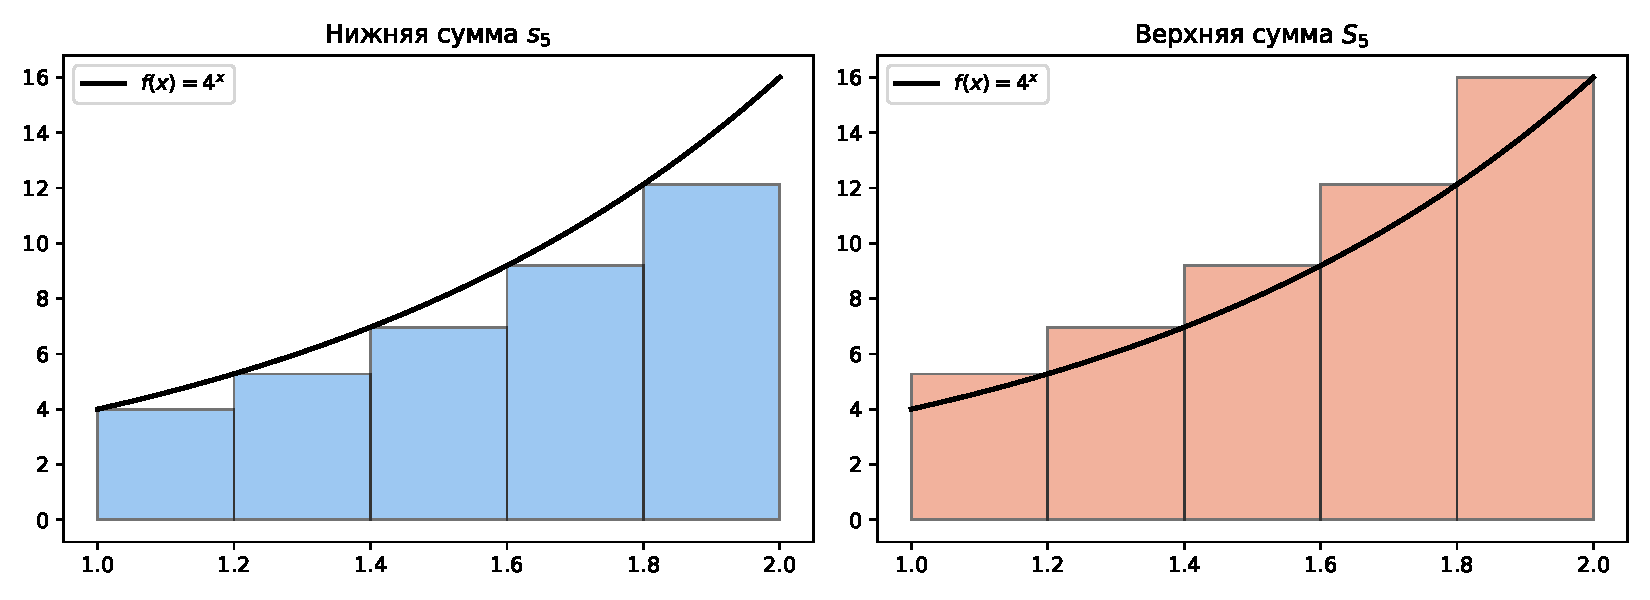
\includegraphics[width=\linewidth]{g_darboux_n5.pdf}
  \caption{Нижняя ($s_5\approx7{,}5116$) и верхняя ($S_5\approx9{,}9116$) суммы Дарбу, $n=5$.}
\end{figure}

%----------------------------------------------
\subsection{График 2: Суммы Дарбу, $n=10$}
%----------------------------------------------

\begin{figure}[H]
  \centering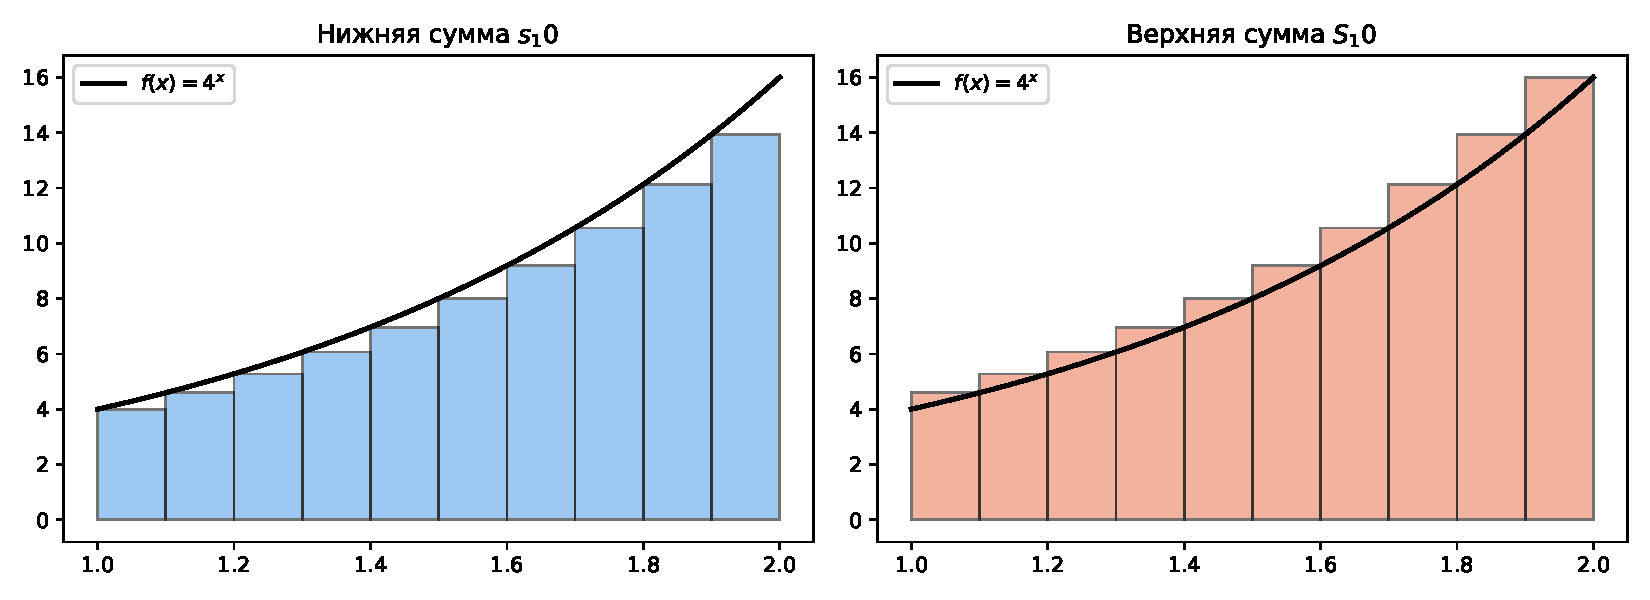
\includegraphics[width=\linewidth]{g_darboux_n10.pdf}
  \caption{Нижняя ($s_{10}\approx8{,}0700$) и верхняя ($S_{10}\approx9{,}2700$) суммы Дарбу, $n=10$.}
\end{figure}


%----------------------------------------------
\subsection{График 3: Суммы Дарбу, $n=100$}
%----------------------------------------------

\begin{figure}[H]
  \centering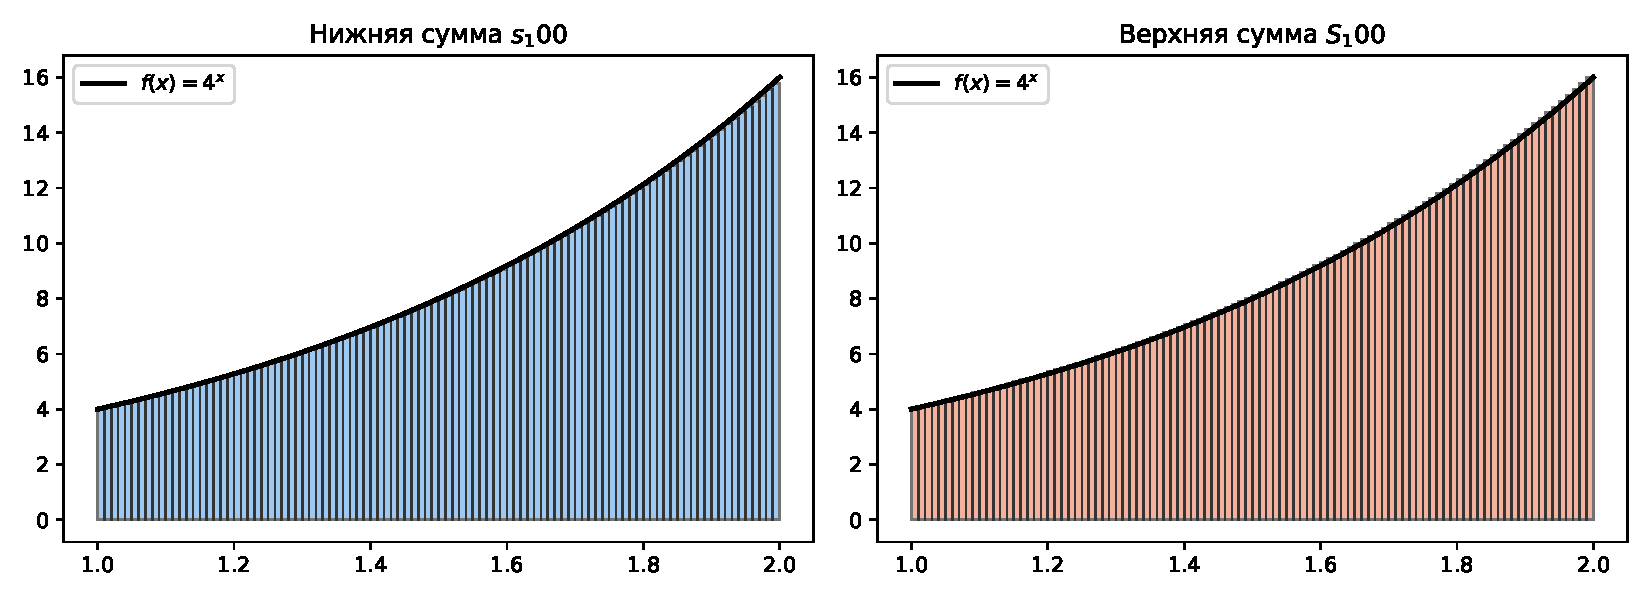
\includegraphics[width=\linewidth]{g_darboux_n100.pdf}
  \caption{Нижняя ($s_{100}\approx8{,}5963$) и верхняя ($S_{100}\approx8{,}7163$) суммы Дарбу, $n=100$.
           Ступенчатые фигуры практически сливаются с кривой.}
\end{figure}


%----------------------------------------------
\subsection{График 4: Случайные оснащения}
%----------------------------------------------

\begin{figure}[H]
  \centering\includegraphics[width=\linewidth]{g_random.pdf}
  \caption{Суммы Римана со случайными оснащениями $\xi_k\in[x_{k-1},x_k]$
           для $n=5,10,100$.}
\end{figure}


%----------------------------------------------
\subsection{График 5: Метод трапеций}
%----------------------------------------------

\begin{figure}[H]
  \centering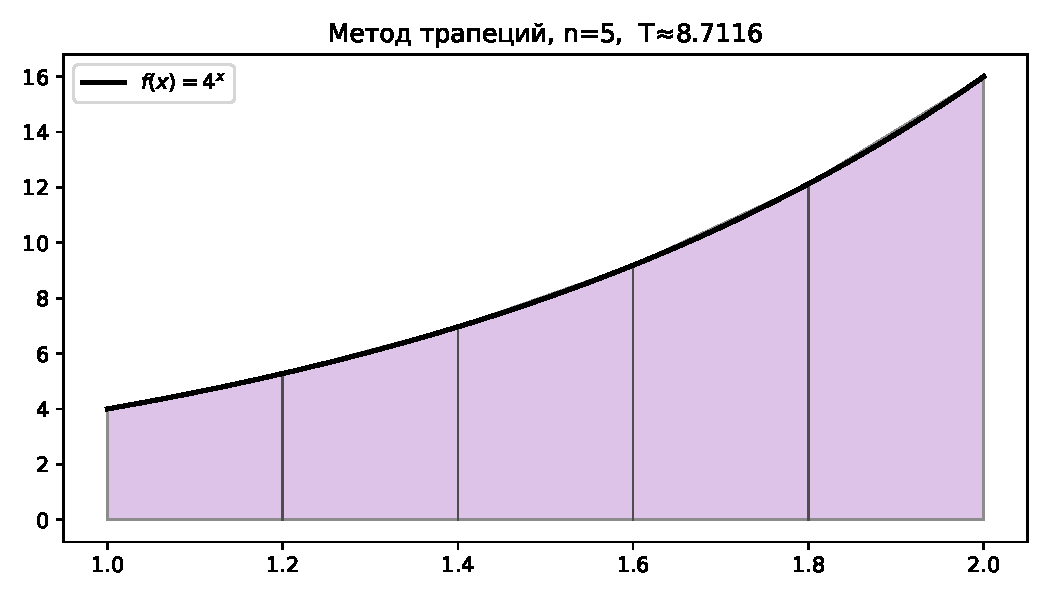
\includegraphics[width=0.62\linewidth]{g_trap.pdf}
  \caption{Метод трапеций, $n=5$: $T_5\approx 8{,}7116$.}
\end{figure}

%----------------------------------------------
\subsection{График 6: Сходимость}
%----------------------------------------------

\begin{figure}[H]
  \centering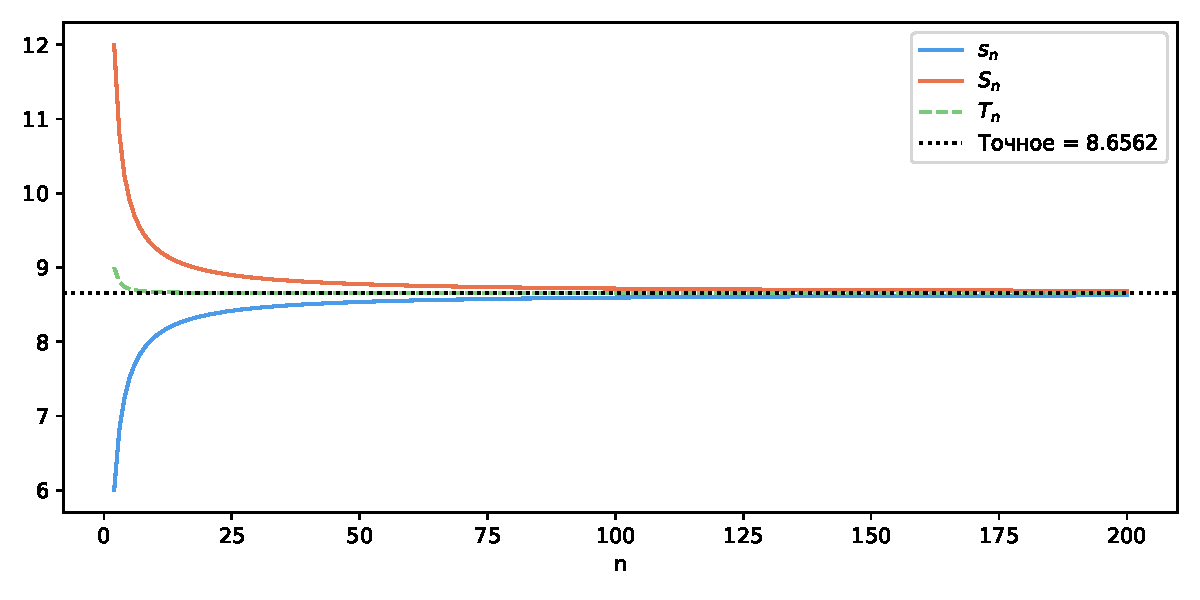
\includegraphics[width=0.85\linewidth]{g_convergence.pdf}
  \caption{Сходимость $s_n$, $S_n$, $T_n$ к точному значению $12/\ln 4$.}
\end{figure}

%----------------------------------------------
\subsection{Таблица численных приближений}
%----------------------------------------------

\begin{table}[H]
\centering
\caption{Приближения $\int_1^2 4^x\,dx=12/\ln 4\approx8{,}6562$}
\begin{tabular}{ccccc}
\toprule
$n$ & $s_n$ (нижняя) & $S_n$ (верхняя) & $R_n$ (случайн.) & $T_n$ (трапеции) \\
\midrule
  5 & 7{,}5116 & 9{,}9116 & 8{,}7093 & 8{,}7116 \\
 10 & 8{,}0700 & 9{,}2700 & 8{,}6810 & 8{,}6700 \\
100 & 8{,}5963 & 8{,}7163 & 8{,}6564 & 8{,}6563 \\
\midrule
$\infty$ & $12/\ln4$ & $12/\ln4$ & $12/\ln4$ & $12/\ln4$ \\
\bottomrule
\end{tabular}
\end{table}

%==============================================
\section{Результаты}
%==============================================

\begin{enumerate}[label=\textbf{\arabic*.}]
  \item Точное значение:
        $\displaystyle\int_1^2 4^x\,dx=\frac{12}{\ln 4}\approx8{,}6562$.
  \item Замкнутые формулы:
        $s_n=\dfrac{12}{n(4^{1/n}-1)}$,\;
        $S_n=s_n\cdot4^{1/n}$,\;
        $S_n-s_n=\dfrac{12}{n}\to 0$.
  \item Интегрируемость доказана двумя способами.
  \item Все численные методы сходятся к $12/\ln 4$.
  \item Формула Ньютона--Лейбница подтверждает ответ. \checkmark
\end{enumerate}

%==============================================
\section{Обсуждение результатов}
%==============================================

\begin{enumerate}[label=\textbf{\arabic*.}]
  \item \textbf{Монотонность упрощает формулы.}
        Строгое возрастание $f(x)=4^x$ означает, что $s_n$ совпадает
        с суммой левых концов, а $S_n$ --- с суммой правых концов,
        что позволяет записать обе суммы через геометрическую прогрессию.
  \item \textbf{Точная разность $S_n-s_n=12/n$.}
        Телескопическое сокращение даёт точную формулу без неравенств.
  \item \textbf{Скорость сходимости.}
        Суммы Дарбу: $O(1/n)$; метод трапеций: $O(1/n^2)$ ---
        заметно точнее при тех же $n$.
  \item \textbf{Стандартный предел.}
        $\lim_{h\to0}(4^h-1)/h=\ln 4$ --- производная $4^x$ при $x=0$
        (Stewart, \S 3.1): связь дифференциального и интегрального исчисления.
  \item \textbf{Согласованность всех методов.}
        $s_n$, $S_n$, случайные оснащения и трапеции --- все стремятся
        к одному значению $12/\ln 4$, подтверждая единственность интеграла.
\end{enumerate}

%==============================================
\section{Используемые программные средства}

Данная лабораторная работа выполнена с использованием следующих инструментов:

\begin{itemize}
    \item \textbf{Python 3.x} --- основной язык программирования для численных расчётов
    \item \textbf{NumPy} --- библиотека для численных вычислений и работы с массивами
    \item \textbf{Matplotlib} --- визуализация графиков и диаграмм
    \item \textbf{LaTeX/XeTeX} --- подготовка научного отчёта
\end{itemize}

\noindent Полный исходный код проекта, включая Python скрипты для численных расчётов 
и генерации графиков, доступен в открытом репозитории на GitHub:

\begin{center}
\url{https://github.com/mohamedellithyyyy/Mathematical-analysis/tree/master/2nd_semester/Lab1}
\end{center}

\end{document}